%!TEX root =  main.tex
%!TEX encoding = UTF-8 Unicode
\chapter{推薦の提示}
\label{chap:output}

本章では,\ref{sec:cfscheme}の推薦システムの実行過程の最後の段階である「推薦の提示」についてまとめる.
この段階では,予測した評価を,活動利用者の目的に適した形式で提示する.
なお,推薦システムの利用者へのアンケート調査結果に基づいて,結果の出力に対する設計指針を,定性的な面から論じた文献に\cite{sigir:01:01}がある.
推薦したアイテムに関する情報も提示すべきことや,推薦リストのレイアウトや,これを閲覧するインターフェースの重要性などを指摘している.

\section{推薦の配送}
\label{sec:present:delivery}

利用者に推薦結果を届ける手段は,次のように分類できる.
\begin{description}
 \item[push型]
 利用者が,システムを直接には使っていない場合に,利用者に推薦を届ける.
 個人化していないバナー広告や,個人化したメールマガジンなどが該当する.
 \item[pull型]
 システムを使用中の利用者が要求したときに,それに応じて推薦結果を届ける.
 検索質問を使う直接指定型の内容ベースフィルタリングの推薦は,この方法を用いる.
 \item[passive型]
 利用者がシステムを使用中に,推薦結果を添付しておく.
 例えば,商品と共に推薦の度合いを★印で示したり,関連商品を同時に示したりする.
 利用者に主導権があり,システム側は積極的な推薦はしない.
\end{description}
\ref{sec:systemtarget}の5種類の運用側の目的のうち「通知サービス」ではpush型を,他の目的ではpull型かpassive型を利用することになる.

その他,配送するかどうかの決定についての工夫もある.
マイクで獲得した発話内容から,視聴中のTV番組への関心の度合いを推定し,関心が低いと推定されたときにのみ積極的に推薦をする方法\cite{trjsai:07:01}などが提案されている.

\section{推薦アイテムの選別}
\label{sec:present:selection}

予測評価の高いアイテムでも,推薦すべきでないアイテムがある.
そういったものを必ず選別し除外しておく必要がある.

利用者が既知であると分かっているアイテムを推薦してもほとんど意味がないので,これらのアイテムを除外する.
例えば,同じセッション中ですでに提示したアイテムや,購買履歴から過去に購入したことがあるものなどを除外する.
また,非個人化推薦である売上げランキングなどを同時に表示する場合は,重複したアイテムを除外しておく方がよいだろう.
文献\cite{trieice:07:03}では,利用者から,アイテムへの好き嫌い評価だけでなく,既知かどうかの情報も得る.
その情報に基づいて,利用者がアイテムを既知かどうかも予測し,未知と予測されるアイテムをより積極的に提示する.

その他,アイテム,デモグラフィック,およびコンテキストの情報に基づいた除外も必要になる.
例えば,アイテムに依存した条件としては,在庫がないとか,利用者が海外在住で発送できない理由で提供できない商品がある.
当然ながら,違法なアイテムも除外すべきである.
また,色違いなど差異がわずかなのものは,代表的なものをひとつだけ残して,残りは提示しないといったことを行う.
デモグラフィックな特徴は,女性専用の旅行プランは男性には推薦しないといったことに利用できる.
また,コンテキストの情報に関しては,利用者の現在位置から遠いレストランは推薦すべきではないし,夏に冬物衣料をすべきではないといった季節商品の問題もある.

\section{推薦の表示形式}
\label{sec:present:style}

推薦すべきアイテム群を表示する形式は,\ref{sec:recomtask}のタスクの種類に応じて以下のように適切なものを選択すべきである.

\begin{figure}
\centering
\begin{minipage}[t]{0.48\fullwidth}
\centering
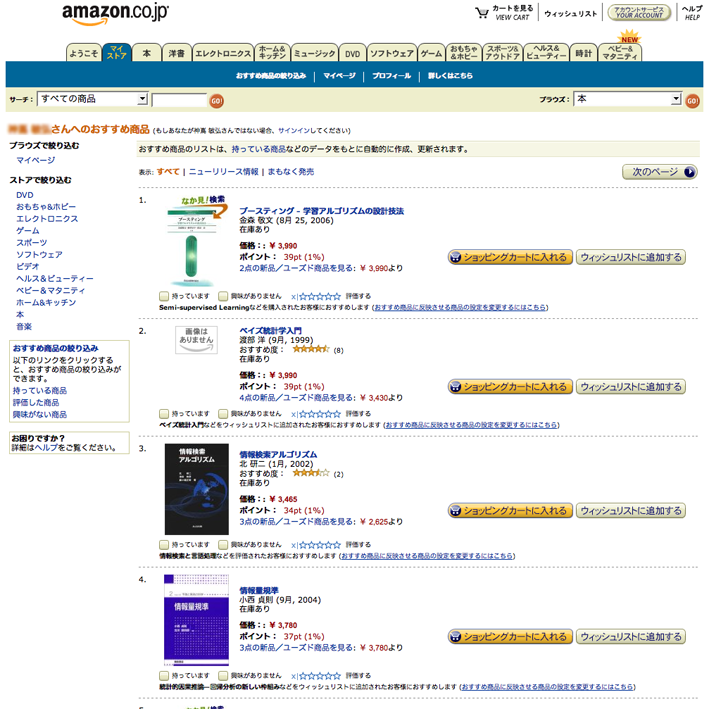
\includegraphics[width=\textwidth]{pstyle1.png}\\
(a) 適合アイテム発見 (Amazon.co.jp)
\end{minipage}
\hspace{0.02\fullwidth}
\begin{minipage}[t]{0.48\fullwidth}
\centering
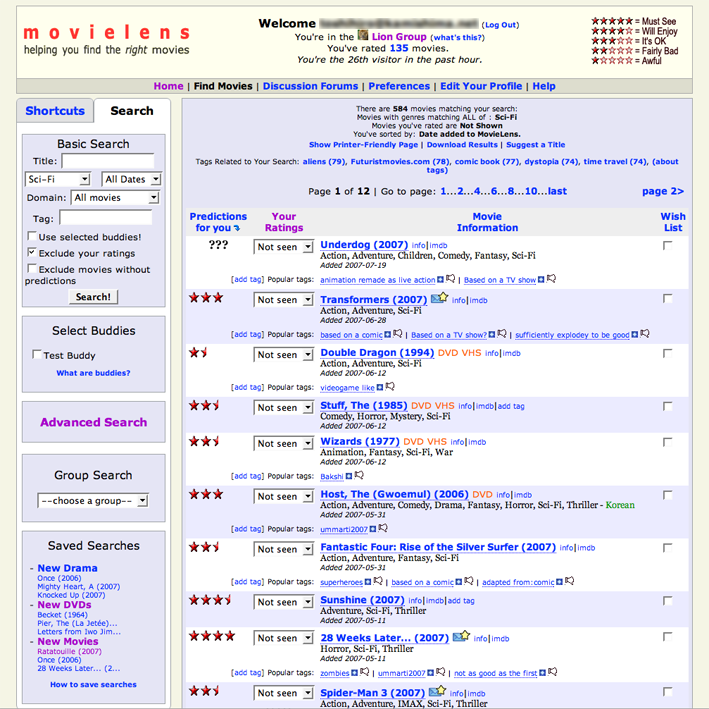
\includegraphics[width=\textwidth]{pstyle2.png}\\
(b) 評価値予測 (MovieLens\cite{url:008})
\end{minipage}\\
\caption{推薦結果の表示例}
\label{fig:presentation}
{\footnotesize スクリーンショットは 2007/07/26 に取得した.}
\end{figure}

適合するものを一つ見つけ出す適合アイテム発見を目的とする場合には,予測される評価の高いものから順に整列したリストを利用者に提示するのが一般的である(\ref{fig:presentation}(a)).
%このリストの上位のアイテムほど,利用者の嗜好に適合する確率が高いだろう.
利用者はこのリストを上位から閲覧することで,自分の嗜好に適合したアイテムを素早く見つけることができる.

評価閲覧を目的とする利用者は,積極的な決定をする意図をもっていない.
そこで,閲覧中のアイテムに,活動利用者の予測評価値を付随的に提示する.これは,★の数や,アイコン,グラフなどで表す(\ref{fig:presentation}(a)).
このような情報を参照することで,多数の候補の中から,利用者にとって関心のあるものを中心に閲覧できるようになる.

%利用者が自分の嗜好に適合するものを網羅的に見つけ出すことが目的である,適合アイテム列挙では,全ての候補を必ず利用者に提示しなくてはならない.

\section{多様性の向上}
\label{sec:serendipity}
\index{多様性}\index{diversity}
%@@@ 多様性の章に移行

評価閲覧(\ref{sec:recomtask})を目的とする場合は,利用者の関心の幅を広げるため,多様性(\ref{sec:recomtype})の高い推薦
が望まれる.
そこで,文献\cite{www:05:01}では多様性を向上させる目的で,予測精度を犠牲にしても,より広範囲の分野のアイテムを推薦する\term{話題多様化}{topic diversification}を提案している.
この多様化の有効性を,同種のアイテムに対しては,1度目より2度目,2度目より3度目に支払いたいと思う対価が減少する経済学における収穫逓減の法則 (law of diminishing marginal returns)との関連付けて論じている.
具体的には,アイテムの階層的な分類を導入し,分類階層の近さによってアイテム間の類似度を測る.
純粋に予測精度を重視したリストの上位から順に,最終推薦リストにアイテムを一つずつ追加するが,このとき,すでに推薦したアイテムと類似しているアイテムは推薦されにくいようにする.
この方法により,予測精度を犠牲にして,アイテムの多様性をより重視するような推薦をする実験を行った.
予測精度を単調に減少させ,徐々に多様性を高めると,最初は利用者は推薦の多様性の高まりを認知できたが,ある程度以上になると認知できなくなった.
よって,推薦リストの多様性を利用者が認知できる程度にとどめれば,予測精度もそれほど低下せず,利用者の満足は高まると報告している.
その他,推薦リストに,新製品やあまり知られていないアイテムを必ず混ぜるといった手法も考えられる\cite{sigir:01:01}.

\section{推薦理由}
\label{sec:explanation}
%@@@ 独立した章に

利用者は,不必要に高価なものを薦められていると疑ったりするため,推薦したアイテムを必ずしも採用するわけではない.
採用されない推薦は無意味なので,推薦ができるだけ採用されるような工夫が必要である.
そうした工夫として,アイテムの\term{推薦理由}{explanation of recommendations}も示すことが有効とされている.

文献\cite{sigchi:02:01}では,推薦の\term{透明性}{transparency}と利用者の推薦結果に与える印象との関係を調査している.
ここでいう透明性とは,利用者の入力した評価やその他の情報と,出力された推薦との間の因果関係が明確に説明されていることである.
この調査では,12人の被験者に5種類の商用音楽推薦システムを利用させた.
そして,推薦されたアイテムを好むか,推薦は信頼できるか,そして推薦に透明性があったかの質問をした.
調査の結果は,透明性があると考えた場合の方が,そうでない場合に比べて,有意に推薦された結果を好み,また,その結果を信頼できると答えた.
さらに,推薦されたアイテムを,(a)知らない場合,(b)知っていてかつそれを好きな場合,および(c)知っていてかつそれを嫌いな場合に分け
た.
推薦されたアイテムを好むかどうかの質問については,(b) (a) (c)の順に好んだ.
さらに,(a)と(b)の推薦については,推薦に透明性があると,ないときよりも,有意に推薦されたアイテムを好んだ.
しかし,(c)の推薦については,有意な差はなかった.
これらのことから,利用者が推薦に透明性があると考えたときには,推薦されたものをより好み,その推薦を信頼する.
また,知っている好きなアイテムを推薦されると,推薦に透明性があると利用者は考えるといえる.
なお,実際がどうであるかにかかわらず,透明性があると考えたかを利用者に質問した結果であること,また,システムがデータをねつ造していない点については,利用者はシステムを信頼していることには注意されたい.
利用者もおそらく知っているであろう,一般に知られたアイテムを推薦して,利用者の推薦への信頼を向上させるといったこともできる\cite{sigir:01:01}.

\begin{figure}
\centering
\begin{minipage}[b]{0.48\fullwidth}
\centering
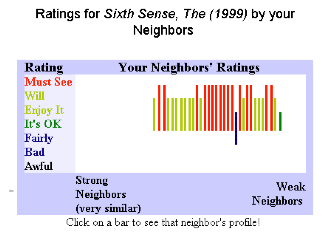
\includegraphics[width=\textwidth]{Herlocker.png}\\
(a)~類似した嗜好の利用者の評価の提示 \cite{cscw:00:01}
\end{minipage}
\hspace{0.02\fullwidth}
\begin{minipage}[b]{0.48\fullwidth}
\centering
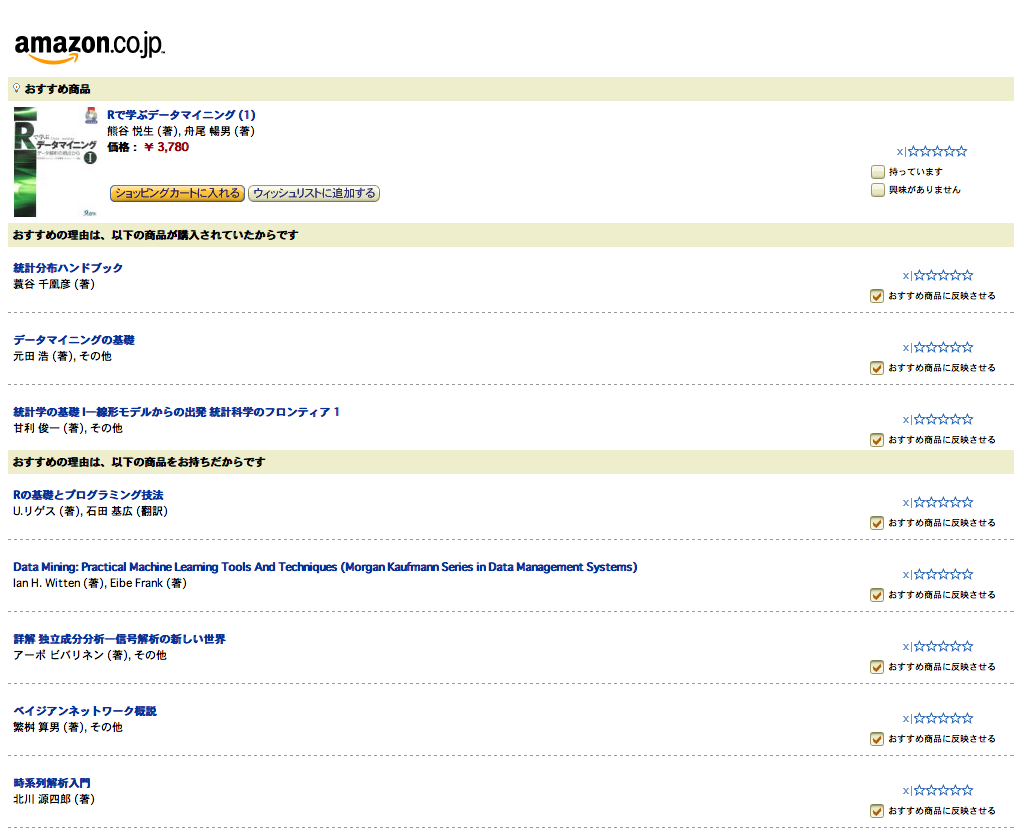
\includegraphics[width=\textwidth]{explanation2.png}\\
(b)~推薦の根拠となった嗜好データの提示 (Amazon.co.jp)
\end{minipage}\\
\caption{推薦理由の提示例}
\label{fig:explanation}
{\footnotesize スクリーンショットは 2007/07/26 に取得した.}
\end{figure}

推薦の透明性を高める,すなわち,利用者が入力した嗜好データから,推薦を導いた根拠を明示することで,推薦への信頼を高める試みがある.
文献\cite{cscw:00:01}では,こうした根拠を提示する手法を比較している.
その中で最も有効な方法とされたのが\ref{fig:explanation}(a)の方法である.
これは,活動利用者と類似した嗜好をもつ他の利用者の,推薦した映画についての評価値を棒グラフで示したものである.
この例では,推薦した映画について,嗜好が似ている人たちのほとんどが,最高か,それに次ぐ評価をしていることが,一目で分かる.
このように,推薦の手順の内部を示すアプローチを\term{ホワイトボックス}{whitebox}アプローチと呼ぶ.
その次に有効であったのは,そうした手順を示さない\term{ブラックボックス}{blackbox}アプローチの,推薦の確信度を示すことであった.
ここで,推薦の\term{強度}{strength}と\term{確信度}{confidence}について述べておこう.
推薦の強度とは,どれくらいアイテムを好むと予測しているかということである.
利用者の嗜好を5段階で予測するなら,5と予測したときに強い推薦といえる.
一方の推薦の確信度とは,この推薦をどれくらい確かだと考えているかということである.
\ref{sec:probmodel}の確率モデルで,適合/不適合の2段階で活動利用者の嗜好を予測したとしよう.
このとき,適合すると予測した確率が$0.6$でも$0.9$でも,予測は「適合」だが,後者のときにより確かな推薦といえる.
さらに,他の方法でも実験したが,利用者の満足を向上させた方法は無かったと報告している.

その他,\ref{sec:item-item}のようにアイテム間の類似度に基づく推薦では,推薦に関連したアイテムを提示するというホワイトボックスアプローチもある.
\ref{fig:explanation}(b)は,活動利用者自身の,推薦の根拠となった他のアイテムへの評価を提示したものである.
また,暗黙的に嗜好データを獲得した場合,推薦の根拠を利用者が認知できなくなるので,推薦と共に根拠となった嗜好データを示す方法もある.
ただし,予測評価値などを提示して,利用者が嫌いなアイテムが高評価されていると,システムに対する信頼を失う危険性も指摘されている\cite{sigir:01:01}.
